\chapter{Conclusion}
In this thesis work we have given a general overview of what authorship attribution is and how it can be addressed with acceptable results nowadays.
We first saw the various types of tasks that can be addressed: instance-based versus profile-based approach. We also saw the differences of single domain documents or previous work on cross domain datasets. We also saw the difference between closed and open set of authors.
We listed the main information retrieval techniques for representing and extracting useful text information, including tf-idf and bag of words, as well as doc2vec.
In Chapter 4 we then listed in detail the state of the art work on authorship attribution and the corpora used, as well as the main classifiers. We have seen how SVM is widely used among machine learning models for some of its peculiar features (including the speed of training and the scalability as features increase). We also showed how Reuters Corpus and The Guardian datasets are the most used datasets for autorship attribution work.
In chapter 5 we have described the work we have done starting from the preparation of the dataset, the selection and extraction of features and finally the choice of the model using an automatic optimization tool (TPOT).
In the last chapter 6 we showed the best metrics obtained with our approach, comparing them also with results obtained reproducing the same scenario of related works.
We showed how for the RCV1-10 dataset we improved to the best of our knowledge by 6.71\% the accuracy of the model compared to the best result obtained with using local histograms. We also improved the RCV1-50 dataset by 6.11\% over the best result obtained using a doc2vec word model.
We then also reported results for 4 total datasets, including a dataset of Victorian-era books collected by the GDELT project and the amazon food reviews dataset, which showed the best results in terms of accuracy among the top 3 datasets that are united by number of authors and number of documents in training and testing.
We then also showed how our approach did not show significant improvements on The Guardian corpus dataset, thus proving suboptimal cross domain and cross topic performance.


In this work we mainly focused our efforts towards author attribution in its most straightforward form, i.e. we are given examples of the writing of a number of candidate authors and are asked
to determine which of them authored a given anonymous text \cite{koppel2009computational}.
This approach to author attribution has been the only one studied until the last decade, as it is already quite complex.
The enormous steps forward both in terms of modern computing power and in terms of studies of new models of machine learning, have allowed us to leave the concept of classical attribution and explore some of the tasks still unsolved. 

\paragraph{The open set authorship attribution} One of the closest problems to being solved in this field of authorship attribution is undoubtedly moving from a closed set group of authors to an open set group of authors. This revolution in approach allows us to have a group of authors in the supervised training phase and a classifier who must take into account that in the testing phase it may have to deal with labels (i.e. authors in this case) that it has never seen in the training phase and classify them as unknown. This approach is complex because it puts together similarities between the verification problem and the needle-in-haystack problem with the classic approach of author attribution in a closed set.
During the study of our work we have tried to validate our approach by dealing also with a type of open set of author attribution.
In fact, we removed 10\% of the authors from each dataset in the training phase and moved them to the testing phase.
To give the reader a better understanding we show a practical example: for the dataset RCV1-50 with 50 authors, for each of them we collected 100 documents.
In the closed set authorship attribution approach we would have had a 50/50 split, i.e. 50 documents of each author would have gone in the training phase and 50 documents of each author in the testing phase, thus leading to a balanced splitting between the classes.
In the open set authorship attribution approach, we selected 5 of the 50 authors whose 100\% of the documents (i.e., 100 documents) we placed in the testing phase by moving them out of the training phase. We thus obtained an unbalanced splitting of classes with a total of 50 documents for 45 authors in the training phase (a total of 2250 documents) and 50 documents for 45 authors, adding 100 documents for each of the 5 remaining authors in the testing phase, ending up with a total of 2750 documents in the testing phase.
For the open set authorship attribution approach we used a One Vs Rest classifier from the python library $
sklearn.multiclass.OneVsRestClassifier$ i.e. we built a classifier for each author, giving his 50 documents as positive examples and all other documents belonging to the other authors as negative examples.
We then inserted an additional label in the training phase, marking it as \enquote{unknown author} for the testing phase.
The results obtained with the datasets selected in this work are shown in \autoref{fig:results_open_set}. We excluded the dataset from The Guardian Corpus as the number of authors in the full dataset was too small to allow for reliable results without introducing learning bias.

\begin{figure}[ht]
	\centering
	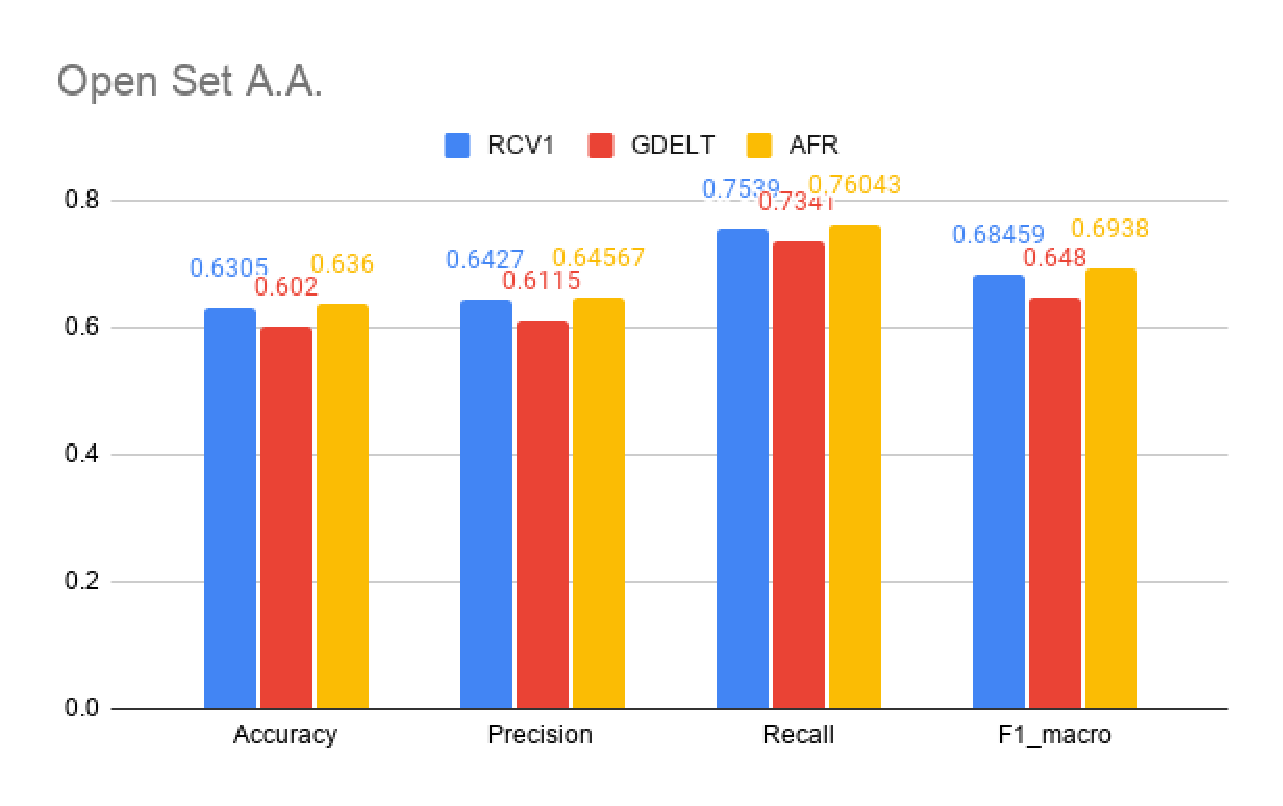
\includegraphics[width=1.0\textwidth, height=1.0\textheight, keepaspectratio]{open_set_aa}
	\caption[Results of our single topic dataset with open set authorship attribution]{Accuracy, precision, recall and f1-macro for Reuters Corpus, GDELT corpus and Amazon Food Reviews corpus for the open set authorship attribution task (10\% of unknown authors).}
	\label{fig:results_open_set}
\end{figure}

As we can see from the results obtained, there is a lot of room for improvement in terms of accuracy. In fact, we obtained results up to almost 25\% lower than the values obtained for the datasets considering the closed set authorship attribution problem.
These considerations made us mainly focus on the classical approach, but they give us the idea that many studies could come out on this particular type of authorship attribution subtask in the next years, as we have not yet found a valid approach that works for all types of datasets and for different authors set size.
